% Setup - do not change
\documentclass[11pt]{article}
\usepackage[top=0.9in, left=0.9in, bottom=0.9in, right=0.9in]{geometry} 
\usepackage{parskip}

\usepackage[english]{babel}
\usepackage[utf8]{inputenc}
\usepackage{amsmath,amsthm,amssymb,graphicx,pdfpages,lipsum,hyperref}
\usepackage{subcaption}
\usepackage[none]{hyphenat}
\usepackage{csquotes}

\setlength\parindent{0pt}
%%%%%%%%%%%%%%%%%%%%%%%%%%%%%%%%%%%%%%%%%%%%%%%%%%%%%%%%%%%%%%%%%%%
% add other packages here if required

%% Bibliography are specified in this file. You can also choose inline bib style if you want to. But make sure your citation style is consistent (and proper)
% For more details on citation: https://library.unimelb.edu.au/recite
\usepackage[sorting = none]{biblatex}
\addbibresource{references.bib}

%%%%%%%%%%%%%%%%%%%%%%%%%%%%%%%%%%%%%%%%%%%%%%%%%%%%%%%%%%%%%%%%%%% the '%' symbol denotes comments

% Begin document creation
% DELETE THE \lipsum PLACEHOLDERS WHEN YOU BEGIN
\title{\textbf{Impact of Shootings on Green Taxis in New York City}}
\author{
Ramon Javier L. Felipe VI \\
%% Replace the link with your github repo
% 1. Remember to escape underscore (\_) in the link.
% 2. Remember to include the commit you want to submit in the link
\href{https://github.com/raja-felipe/taxi-crime-analysis}{Github repo with commit}
}

\begin{document}
\maketitle

\section{Introduction}
% Link to a 30 min tutorial if you require revision: https://www.overleaf.com/learn/latex/Learn_LaTeX_in_30_minutes
Shootings are becoming increasingly prevalent in the United States, and New York City is no different. As of August 1 this year, over 25,000 people have died of gun violence \cite{2023shootings}. Even if shootings decreased by 25\% in New York this year, the fact that over 3,424 guns and 2,162 gun arrests occurred in June 2023 alone should emphasize how rampant gun violence has become \cite{nyc25}. Cases of bullets hitting riders on a normal everyday ride demonstrates a real and probable danger anyone living in this area has to prepare for\cite{friendshooting}. 

It would be crucial for green taxi drivers to better understand this phenomenon and how it affects consumer demand. For the past few years, the number of green cabs have been plummeting, decreasing to a mere 900 now from 6,500 in 2015. \cite{greenlose}. Shootings may further exacerbate this situation, so it is crucial for stakeholders, like taxi drivers, to grasp a better understanding of the impact of shootings on green taxis. 

The paper will thus present two different time series models to forecast a future day's consumer demand based on green taxi rides in New York City per day and historic New York Police Department (NYPD) shootings data. Asides from benefiting taxi drivers who would like to know when a shooting significantly affects their demand, it can also help stakeholders understand the true nature of shootings as a naturally occurring event. In a country where such tragedies are slowly becoming more normalized, knowledge of the relationship between taxis and shootings can mean life or death for some people.

% Example here used biblatex to manage citations: https://www.overleaf.com/learn/latex/Bibliography_management_with_biblatex , You are free to choose your own way for managing references if biblatex seems too hard.


% You can have \section{}, \subsection{}, and \subsubsection{}, \section*{}, \subsection*{}, and \subsubsection*{}
\section{Dataset}

The main dataset selected for this research is the \textbf{Taxi Limousine Commission (TLC) Taxi Trip Record Data} of green taxis \cite{tlc}. This contains recorded trips made by green taxis. Various characteristics are stored in this dataset, such as time, location, fees, and taxes. Contextually, the COVID-19 pandemic caused a significant rift in the overall trend of both taxi demand and shootings. This decision led the researcher to lean towards data from and after 2022 since this would be when the pandemic confidently ended.

The other dataset regarding shootings was taken from the \textbf{New York Polic Department (NYPD)} \cite{nypdshootings}. This stores data on all recorded instances of shootings from history, so the dataset goes as far back as pre-2000s. Similar to the green taxi data, the pandemic has significantly altered the trends of shootings compared to pre-pandemic ones. Thus, the researcher also assumes these trends differ enough significantly to warrant uncertainty about the relevance of past trends. Similar to the taxi data as well, only shootings data from 2022 and later would be used.

Table 1 below summarizes the shapes of both of our datasets. There is a significant difference in size between the datasets which should be contextually true. Shootings would and should not be as frequent as taxi trips. This is an important factor that will be addressed later in modelling.
\begin{table}[h]
	\begin{center}
		\begin{tabular}{|l|l|l|}			
			\hline
			Dataset & Instances & Rows\\
			\hline\hline
                Green Taxis & 285537 & 22 \\
			Shootings & 1716 &21\\
			\hline
		\end{tabular}
		\caption{Shape of Datasets}
		\label{table1}
	\end{center}
\end{table}

\section{Preprocessing}

Preprocessing for the datasets in this research mainly involved handling missing values and adhering to explicit and implicit business rules. It must be noted that there were columns in both datasets that were dropped immediately because too many of the entries were missing. For the taxi data, these were \textbf{congestion surcharge} and \textbf{ehail fee}. For the shootings data, these were the \textbf{features concerning the shooter} and the \textbf{specific details of the shooting location}, such as whether it was a house or a park. After removal of these columns, it is safe to remove rows with missing entries in both datasets.

\subsection{Green Taxi}
For the green taxi data, there were many nuances and business rules based on the data dictionary. Those rules were followed, but a few more conditions were added as a result of the researcher's interpretation of the business rules and adherence to his research aim.
\begin{itemize}
    \item\textbf{Location IDs} should be from 1 to 263. Additionally, green taxis are not allowed to pick up from Yellow Zones.
    \item\textbf{Trip Distance and Trip Duration} cannot have negative distances and time taken respectively.
    \item\textbf{Passenger Count} cannot be negative or zero. The only trips in the data set concerning the research are trips with passengers since these trips will be the most impacted by a given shooting.
    \item \textbf{Payment Amounts} should not be negative, like fare amount and tolls amount.
    \item \textbf{Tip Amount} does not include cash tips. From the data dictionary, the other payment types such as ``unknown`` or ``voided trip``. Hence, the research will assume that all non-credit card payments should have a tip amount of zero.
    \item \textbf{Improvement Surcharge}  can only be 30 cents, and only applicable to trips that were hailed. The research assumes that if the trip was not hailed, this value can only be zero.
    \item \textbf{Date and Time} has to be within 2022 to 2023.
\end{itemize}

Enforcing all these rules and conditions brings us from 1,180,019 entries to just 20,967. Duplicates were not considered in this case because there is no unique ID that can be used to differentiate trips in the taxi's feature set.

\subsection{Shootings}
For our shootings data set, there was very little filtering to do other than account for the use of key words such as ``UNKNOWN`` and ``(null)`` to indicate a missing value. Other than that, null values were also dropped to bring the number of total and duplicates were removed. This reduces the number of shootings from 9,778 entries to just 1,536 entries.

\subsection{Feature Selection}
Out of the features in the taxi data set, only these were selected:
\begin{itemize}
    \item \textbf{Pickup and Dropoff Location IDs}
    \item \textbf{Hour of the Day}
    \item \textbf{Day of the Week}
    \item \textbf{Pickup Date}
\end{itemize}
On the other hand, day of the week, date, and hour of the day were also selected for the shootings data, but there are also other features of importance:
\begin{itemize}
    \item \textbf{Flag for Murder}
    \item \textbf{Victim Sex, Age, and Race}
\end{itemize}
These features were selected as they provide very important context within a given trip or shooting, more so than the other possible options, particularly the time of a taxi trip, location in New York City, and nature of a given shooting. These will all be used to predict the target variable: The number of taxi trips for a given day.

\subsection{Taxi Location IDs Selection}
As there are many possible Taxi Location IDs, the researcher wanted to identify key locations where shootings are of high likelihood. To do this, after the previous steps, the shootings data was aggregated by taxi location ID and a threshold of $>= 30$ shootings to filter out key locations. This significantly reduces the dimensionality of our eventual data set and consequently increases runtime speed and decreases noise. These taxi location IDs are 35, 74, 42, 177, 168, 61, 225, 78, 159, and 169. These will be explained more in detail in the next section.

\subsection{Aggregation and Join}
Each data set was aggregated by their date to create a sequence of days to estimate a trend in the taxi demand based on shooting data. This was to reduce the sparsity of the data set, since shootings by nature are not that frequent. The join also conditioned on a shooting and taxi instance's location IDs, so a match on either the pickup or drop off location ID. Regardless of whether someone moves away or towards a shooting, the incident is enough to impact taxi demand on that day. This process resulted in only 133 joined rows.

It is also important to note that after preprocessing, all data from 2023 was filtered out, with the latest remaining date being December 28, 2022.
 
\section{Preliminary Data Analysis}
\subsection{Geospatial Data Analysis}
Figures 1 shows the trends of taxi rides and shootings respectively over time.

\begin{figure}[h]
    \begin{subfigure}{0.5\textwidth}
        \centering
        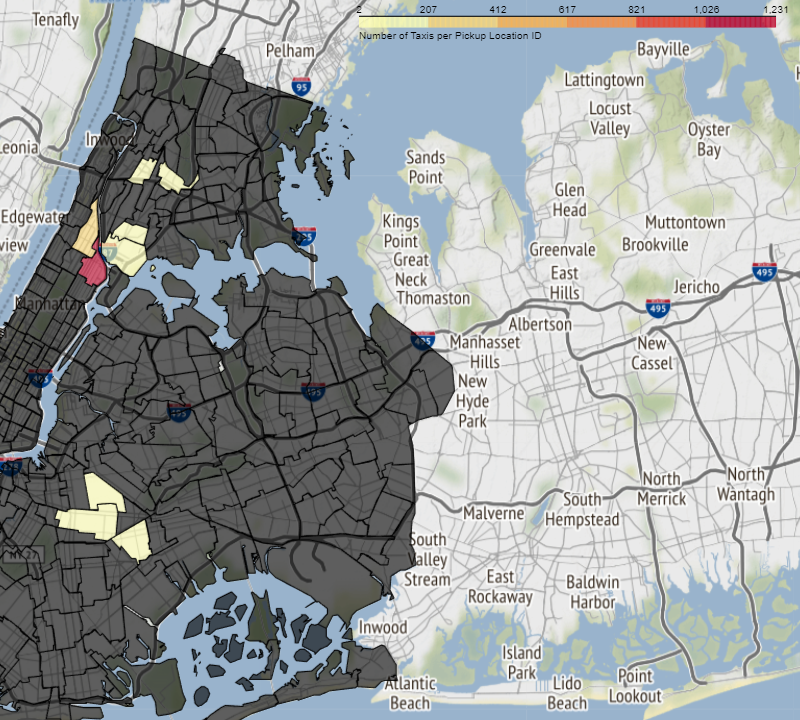
\includegraphics[width=0.8\linewidth]{plots/map_taxi_pickups.png}
        \caption{Green Taxi Demand by Pickup Location IDs}
    \end{subfigure}%
    \begin{subfigure}{0.5\textwidth}
        \centering
        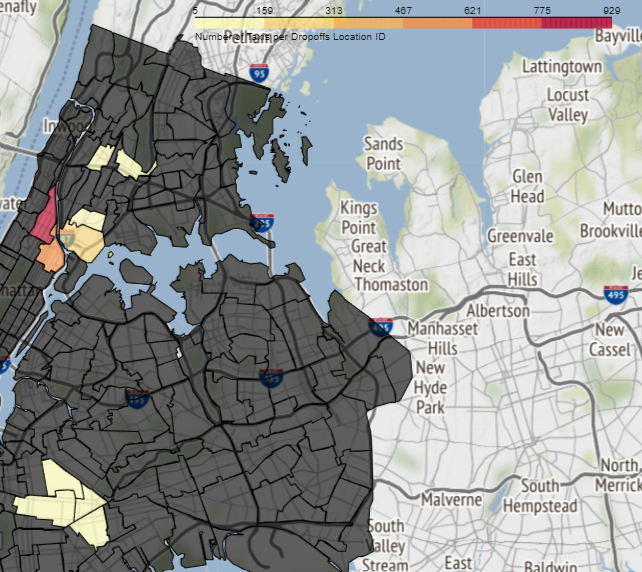
\includegraphics[width=0.8\linewidth]{plots/map_taxi_dropoffs.png}
        \caption{Green Taxi Demand by Dropoff Location IDs}
    \end{subfigure}
    \caption{Green Taxi Demand Comparison between Pickup and Dropoff Locations}
\end{figure} 

The demand for taxis, when considering only where shootings occur, seemed to center entirely around area 74. There were multiple parks nearby, such as Jefferson Park, Wagner Playground, and Crack is Wack Playground. Table 2 tells us that there is a significant jump in shootings from areas ranking lower than 74.  There are just some areas however that were not parks, like Liberty Island. Nonetheless, this trend of parks is consistent with most of the other location IDs. This characteristic leads to a chilling observation. Many of the shootings taxis end up stumbling upon involve large groups of children. This is very believable, considering incidents like the Sunset Park shooting \cite{sunsetpark}.

\begin{table}[h]
	\begin{center}
		\begin{tabular}{|l|l|}			
			\hline
			Location ID & Number of Shootings\\
			\hline\hline
                74 & 1231 \\
			42 & 396\\
                61 & 44 \\
                159 & 40 \\
			\hline
		\end{tabular}
		\caption{Head Rows of Location IDs and Number of Shootings in 2022-2023 in Descending Order}
		\label{table1}
	\end{center}
\end{table}

As for shootings, Figure 2 has the same trend of very concentrated areas, but the numbers are distributed differently, as shown in Table 3. The same trend also exists for shootings. These high risk shooting areas are around parks and consequently children.

\begin{figure}[ht]
    \begin{minipage}{0.5\linewidth}
        \centering
        \begin{tabular}{|l|l|}
            \hline
            Location ID & Number of Shootings \\
            \hline\hline
            159 & 33 \\
            78 & 34 \\
            225 & 35 \\
            61 & 36 \\
            \hline
        \end{tabular}
        \captionof{table}{Head Rows Location IDs \& \# of Shootings in 2022-2023}
        \label{table1}
    \end{minipage}%
    \begin{minipage}{0.5\linewidth}
        \centering
        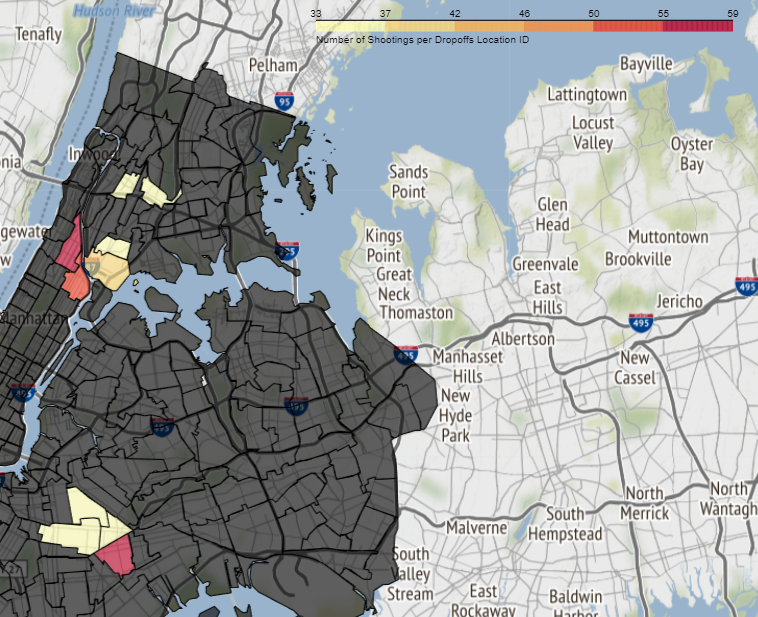
\includegraphics[width=\linewidth]{plots/map_shooting_locs.png}
        \caption{Number of Shooting Incidents by Taxi Location ID}
        \label{fig:shooting-map}
    \end{minipage}
\end{figure}

\subsection{Taxi Demand Trend Analysis}

\begin{figure}[h]
    % change the scale multiplier to make the figures smaller or larger
    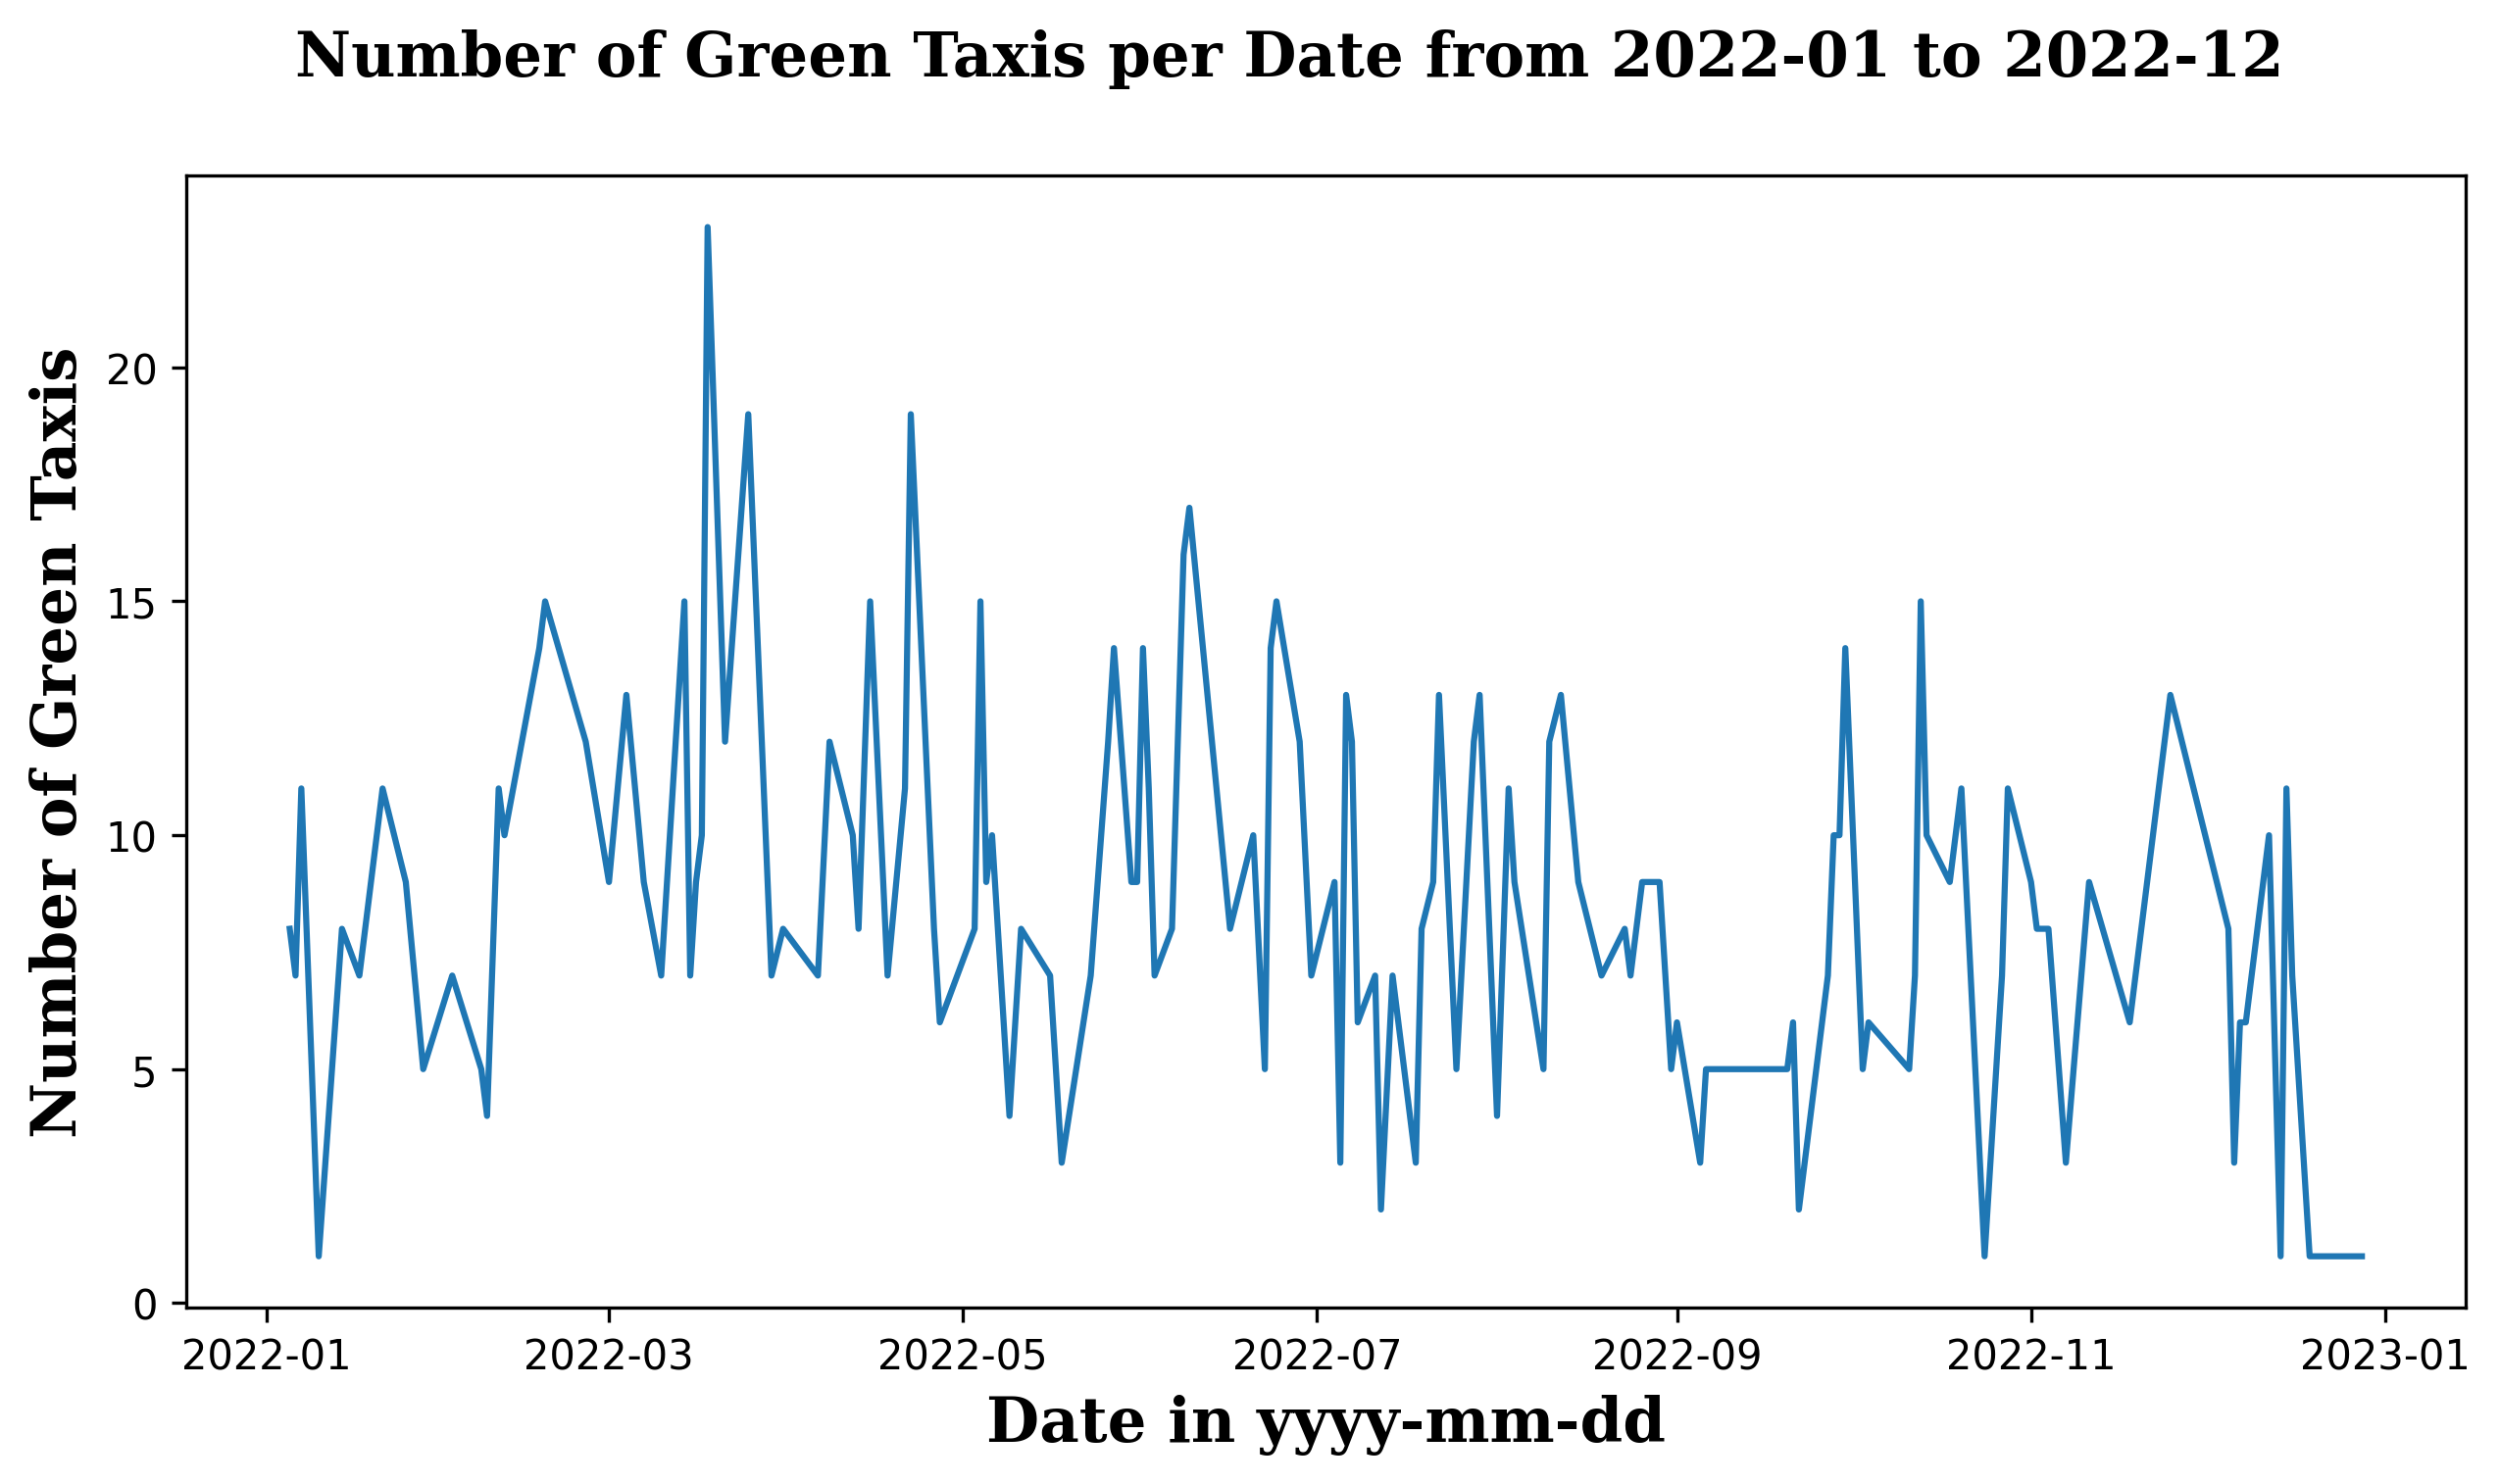
\includegraphics[width=0.65\textwidth]{plots_new/green_per_date_modelling.png}
    % this ensures your figures are centered where possible
    \centering
    \caption{Trend of Number of Green Taxis by Day from 2022 and Later in Aggregated Model} % refer to this image as (Figure 1)
\end{figure}

Looking at Figure 3, the data demonstrates two key ideas about the taxi demand trend within this time range. First, the dataset's trend is relatively stable. Although there are rises and drops over time, it is nothing too different from the trend of the data. Second, achieving a good fit for this model risks overfitting the dataset significantly since the variance of the values is high. 

\section{Time Series Models}

Two time series models were used: a Random Forest Regression and an Autoregressive Integrated Moving Average (ARIMA) Model. These would forecast the demand of taxis at some date in the future. The size of our dataset was extremely small, so no division by a feature could be performed. This scenario was still desirable because shootings are not very regular events, so division into groups would introduce more sparsity. Our data does not have all 133 consecutive days from January 5, 2022. Despite this, the model is still viable because contextually consecutive shooting data is highly improbable. 

These models were trained on 80 instances ranging from January 5 - July 28, 2029, hyperparameter tuned on 27 instances ranging from July 29, 2029 - October 4, 2022, and then tested on 26 instances ranging from July 30, 2029 - December 28, 2022.


\subsection{Random Forest Regression}

Random Forest Regressions are an ensemble modelling technique that uses multiple decision trees trained on different subsets of features and collectively decide on a prediction using methods like mean or mode. \cite{randomforest}. The use of different decision trees allows the model to capture a variety of relationships as well as perform excellently on sparse datasets. It is important to note that random forests ensemble results because a decision tree itself is prone to high variance. Using multiple trees to reduce variance does not mean the variance itself disappears. 

Tuning the hyperparameters of our model involved a grid search on different sets of these values. Due to the nature of a time series model, an actual cross validation would be difficult because mixing train and validation sets risk forecasting for a in the past not the future. Hence, the process was simplified to use one validation set instead due to computational time required.

Additionally, lag variables were introduced in the RFR to make it more viable for a time series. An arbitrary value of 12 lag autoregressions. Within context, this means the model looks at taxi demand from up to 12 days in the past. This makes sense within context of the research where, in the perspective of a taxi driver, they cannot hide from possible shootings for too long to avoid financial repercussions.

\subsection{Autoregressive Integrated Moving Average (ARIMA)}
ARIMA works similarly to a linear regression model, but assumes dependence of observations relative to a time scale. This dependence is illustrated by the past observations $y$ and past errors $e$. The model is constructed to predict $y$ as follows:\
\begin{center}
    $\hat{y} = \alpha + \phi_{1} y_{t-1} + \phi_{2} y_{t-2} ... + \phi_{p} y_{t-p} - \theta_{1}e_{t-1} + \theta_{2}e_{t-2} - ... + \theta_{q}e_{t-q} + \beta_{1} x_{1},t + \beta_{2} x_{2} + ... + \beta_{m} x_{m}$
\end{center}
Where $p$ and $q$ are hyperparameters for the number of past predictions and errors to incorporate in the model respectively, $\phi$ and $\theta$ are coefficients to the past observations and errors respectively, and $m$ is the number of exogeneous variables $x$ with coefficient $\beta$ \cite{duke}.

$d$ is another hyperparameter that indicates the number of nonseasonal differences required to achieve stationarity. Stationarity here means that a time series' statistical properties such as its mean, variance, and autoregression do not change over time \cite{stationarity}. This hyperparameter is important for determining how to convert a current observation to a past observation. It works using the following formula:

$d: 0 \rightarrow y_{t} = Y_{t}$  \\
$d: 1 \rightarrow y_{t} = Y_{t} - Y_{t-1}$  \\
$d: 2 \rightarrow y_{t} = (Y_{t} - Y_{t-1}) - (Y_{t-1} - Y_{t-2})$  \\

where we denote $y_{t}$ as the $d$th difference of $Y$ at time $t$.

Since a time series model like ARIMA is being used, stationarity should be tested first. Using a Augmented-Dickey Fuller test, $p = 0.000000000000000723479226219799$. Since the test is significant at $p = 0.05$, stationarity can be assumed, so $d$ can be denoted as one. The test asserts that a time series is the opposite of non-stationary, but it does not ascertain that our series is actually stationary. The test result is a safe indicator to assume $d = 1$, or only one difference needs to be done to achieve stationarity.

Hyperparameter tuning was also done using grid search to optimize $p$ and $q$ based on a single validation set.

\section{Discussion}

\subsection{Results}
Root Mean Squared Error (RMSE) was used to test each model's performance. This metric is the easiest to implement and interpret. In the context of our problem, this metric allows us to clearly see how far off a model was from truly predicting the taxi demand for a given day. 

Table 4 demonstrates that the ARIMA model is very superior, nearly 270 times smaller in error than the RFR. The behavior of the trend as well in Figure 5 demonstrates ARIMA is able to keep up with the erratic behavior of the taxi demand in the test set. A plausible reason for this behavior is the nature of ARIMA itself. It works well with smaller datasets and missing data, two key characteristics of this use case \cite{arima}. In this case, ARIMA captures more information as well about the 

RFR had significantly higher error in this problem. In a dataset where the max value for a target variable is somewhere in the low 10's, an error rate of almost 2 can be considered poor. However, looking at the actual predicted set the performance was still good. A key reason a Random Forest could not work is because it performs poorly with small data compared to ARIMA. Theoretically, a Random Forest wants a lot of data because it needs enough variance in the data where each decision tree overfits to a different context represented by a subset of feature values. However, when data is small, this is not the case and the probability that multiple decision trees overfit to the same concept causes an overall overfit to the training data.

\begin{figure}[ht]
    \begin{minipage}{0.5\linewidth}
        \centering
        \begin{tabular}{|l|l|}
            \hline
            Model & RMSE \\
            \hline\hline
            RFR & 1.68132002 \\
            ARIMA & 0.00616308 \\
            \hline
        \end{tabular}
        \captionof{table}{RMSE of RFR versus ARIMA Model}
        \label{table4}
    \end{minipage}%
    \begin{minipage}{0.5\linewidth}
        \centering
        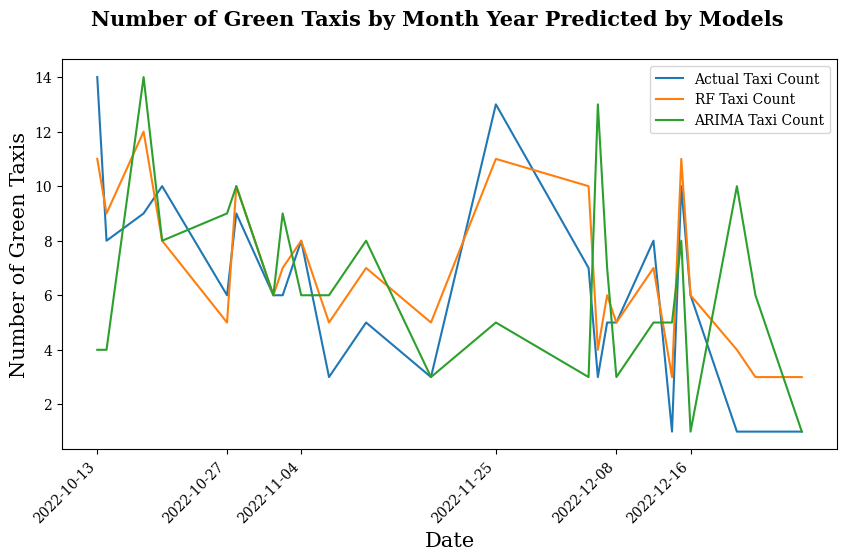
\includegraphics[width=\linewidth]{plots/green_daily_predictions.png}
        \caption{Predictions of RFR and ARIMA Models on Test Set}
        \label{fig:predictions}
    \end{minipage}
\end{figure}

\subsection{Uncertainty Analysis}

Due to the small size of the dataset, it is uncertain whether the performance in the test set is purely coincidental or not. To ascertain this, a cross validation would be ideal, but the nature of a time series does not allow for values set in the past to be grouped with values in the future. A solution is to bootstrap the validation set to create multiple folds that our training set can predict and get the sample variance of the RMSE's calculated. One could also bootstrap the training set. Within contexts of shootings, however,  there would not be a lot of data to work with as they are not normal and frequent occurrences. It is more likely though that a completely different type of shooting occur in the future. Thus, the researcher stuck with this uncertainty analysis. The results of this test further solidify RFR as an unsatisfactory model compared to ARIMA which showed very little variance in the pseudo cross validation.

Table 5 shows the results and again ARIMA possesses significantly lower variance in RMSEs. 
    \begin{center}
    \begin{tabular}[h]{|l|l|}
        \hline
        Model & Variane of RMSE \\
        \hline\hline
        RFR & 1.68132002 \\
        ARIMA & 0.00011549 \\
        \hline
    \end{tabular}
    \captionof{table}{Variance of RMSE of RFR versus ARIMA Model}
    \label{table4}
    \end{center}

\section{Recommendations}

As the ARIMA model can forecast demand of a taxi for a given day with shootings, recommendations for alleviating the struggle of being a taxi driver amidst ongoing or probable shootings is to have companies forecast when taxi demands should be high again. The ARIMA model proved to be strong, especially with the current situation. The pandemic from before has made it difficult to trust forecasts pre-pandemic due to the severe confounding effect it had on previous data's reliability. Rather than possibly risk a taxi driver harm, a predictive model could help drivers know when to be active in case shootings occur based on demand. 

Another recommendation for drivers is to avoid parks as much as possible. The risk of encountering shootings in these areas is significantly higher than other areas in the city. The trend also implies that children populated areas that are outdoors are of significantly higher risk to taxi drivers. If able to, avoiding large crowds of children is ideal.

\section{Conclusion}
The research discussed two time series models to forecast the demand of taxis as number of trips in a day given data regarding time and location of a green taxi trip and characteristics of a shooting incident. ARIMA did significantly better than the RFR model. It is the preferred choice for this specific use case. By incorporating the shooting data into the green taxi data, a unique model was created that could forecast demand of taxis when shootings happen. The model also has other uses cases besides forecasting. It can also be used to interpret and more deeply understand the relationship between taxi trips and shootings. 

For further research, it would be good to investigate other types of crime that could possibly affect the livelihood of taxi drivers such as burglaries. It would also be beneficial to somehow explore larger datasets and more informative datasets. One weakness of the NYPD arrest data was a lot of the perpetrator data was missing, which would have been more informative to taxi demand forecasts than victim data. Overall, a strong model that works for data that will remain relatively small for a while is a good start to better understanding the impact of shooting on taxi demand.


\clearpage

% BEGIN REFERENCES SECTION
\printbibliography

% \begin{enumerate} 
%   \item Example for enumerated points
%    % use \item to create more points
% \end{enumerate}

% \begin{itemize} 
%     \item Example for dot points
%     \item[*] You can change dot points to any symbols by putting [SYMBOL].
%     \item[$\times$] Here's a fun example.
% \end{itemize} 

\end{document}